\documentclass[10pt,xcolor=dvipsnames]{beamer}

\usetheme{default}%simple}

\usepackage{lmodern}
%\usepackage[scale=2]{ccicons}
\usepackage{ccicons}


\usepackage{graphicx}
\usepackage{amsmath,amssymb}
%\usepackage{colortbl}
%\usepackage{color}
\usepackage{algorithm}
\usepackage{algorithmic}
\usepackage{amsthm}
\usepackage{mathtools}   %:= symbol
\usepackage{multirow}
\usepackage{rotating}
%\usepackage[round]{natbib}
%\usepackage[version=0.96]{pgf}
\usepackage{tikz}
\usepackage{tikz-3dplot}
\usetikzlibrary{matrix,calc,shapes,shadows,arrows,positioning,fit}
\definecolor{cof}{RGB}{219,144,71}
\definecolor{greeo}{RGB}{91,173,69}
\tdplotsetmaincoords{70}{165}

\usepackage{amsmath,amsfonts,amscd,amssymb}
%\usepackage[francais]{babel}
%\usepackage[francais]{layout}
\usepackage[english]{babel}
\usepackage[english]{layout}
%\usepackage[utf8]{inputenc}
%\usepackage{nantes_theme}
%\usepackage{multirow}
\usetikzlibrary{calc,3d}
\usepackage{appendixnumberbeamer}

\DeclareMathOperator{\conv}{\rm conv}
\DeclareMathOperator{\cl}{\rm cl}
\newcommand{\mR}{\mathbb{R}}
\newcommand{\mN}{\mathbb{N}}
\newcommand{\mZ}{\mathbb{Z}}
\newcommand{\mB}{\{0,1\}}
\newcommand{\red}{\textcolor{red}}
\newcommand{\blue}{\textcolor{blue}}
\newcommand{\orange}{\textcolor{orange}}
\newcommand{\grey}{\textcolor{black!25}}
\newcommand{\green}{\textcolor{ForestGreen}}
\newcommand{\magenta}{\textcolor{Mulberry}}


%
\newcommand{\R}{\mathbb{R}}%Mengen R
\newcommand{\N}{\mathbb{N}}
\newcommand{\Z}{\mathbb{Z}}
\newcommand{\Q}{\mathbb{Q}}
\newcommand{\ab}{\par\noindent}%Absatz ohne Einzug
%

%\usepackage{berenis}
%\usepackage{schemata}
%\usetikzlibrary{trees}
\usetikzlibrary{mindmap}
%
%\usepackage{microtype}%Zeilenumbruchverbesserung
%\usepackage[T1]{fontenc}%Kodierung der Ausgabe

%\usepackage{biblatex}%Literaturverzeichnis, falls notwendig. Ansonsten auskommentieren
%\addbibresource{Literatur.bib}%Name des Literaturverzeichnises hier einfügen!!!

\usepackage{url}%Anklickbare URL im pdf
%\usepackage{hyperref}%Anklickbare Kapitel im Inhaltsverzeichnis und anklickbare Referenzen; beides im pdf

%\graphicspath{{pictures/}}%Pfad, in dem die Bilder gespeichert sind: Im Unterordner bilder

\usepackage{tabularx}%Tabellen
\usepackage{booktabs}%Verbesserungen und andere Kommandos für Tabellen

\usepackage{units} %Weiteres Mathepaket mit \nicefrac{Zähler}{Nenner} Umgebung für Brüche
\usepackage{eurosym}%Eurozeichen
%\usepackage{csquotes} %Anführungszeichen

%\usepackage{algpseudocode} %Algorithmen

%\usepackage{pgfplots}%Plots
%\usepgfplotslibrary{dateplot}

\usepackage{xcolor}%mehr Farben
%\usepackage{BeamerColor}

\usepackage{xspace}

\usepackage{todonotes}
\usepackage{caption}
\usepackage{subcaption}
%

%\setwatermark{\includegraphics[height=8cm]{img/Heckert_GNU_white.png}}


%
% --- Tikz definitions from Stefan
%
\colorlet{boxfill}{black!10}
\colorlet{boxhead}{black!20}
\colorlet{boxdraw}{black!70}
\colorlet{linescolor}{black!70}
\tikzstyle{boxstyle}=[draw=boxdraw,text=black,thick,rounded corners]
\tikzstyle{taskbox}=[boxstyle,rectangle,text width=3cm,rectangle split,rectangle split parts=2,
                     rectangle split part fill={boxhead,boxfill}]
\tikzstyle{line}=[very thick,linescolor,rounded corners]

%
% --- 1st slide
%

\title{{vOptSolver -- Version 0.2 }}
\subtitle{Software developed with the support of the ANR/DFG-14-CE35-0034-01}
\date{\today}
\author{Universit\'e de Nantes}% -- University of Koblenz-Landau}
\institute{\url{https://github.com/vOptSolver}\\ \url{https://voptsolver.github.io/vOptSpecific/}\\ \url{https://voptsolver.github.io/vOptGeneric/}}
%\titlegraphic{\includegraphics[height=1cm]{logoParis.png}\hfill\hfill\includegraphics[height=1cm]{logoParis.png}\hfill\hfill

%\titlegraphic{\vspace{65mm}\includegraphics{logovopt4.jpg}}

%\pgfplotsset{compat=1.14}


\begin{document}


\maketitle

%
% ================================================================
% 
\begin{frame}{Table of contents}

\begin{itemize}

  \item Introduction to vOptSolver
  \item Instructions for installing and running vOptSolver 
  \item vOptSpecific problem by problem
  \item vOptGeneric problem by problem
  \item Technical overview
  \item History
  \item Taskforce
  \item Links and contact

\end{itemize}
\vspace{10mm}

Convention: \grey{text in grey} $\Rightarrow$ functionality integrated in future releases

\end{frame}

%
% ================================================================
% 
\begin{frame}

\begin{center}
{\Large
 \textcolor[RGB]{52,57,176}{
   Introduction to vOptSolver
 }
} 
\end{center}
\end{frame}

%
% ================================================================
% 
\begin{frame}{Multi-objective linear optimization problems targeted}

{\small
\begin{itemize}
\item LP: Linear Program
\item MILP: Mixed Integer Linear Program
\item IP: Integer Linear program
\item CO: Combinatorial Optimization
\item LAP: Linear Assignment Problem
\item OSP: One machine Scheduling Problem
\grey{
\item UKP: Unidimensional 01 Knapsack Problem
\item MKP: Multidimensional 01 Knapsack Problem
\item UFLP: Uncapacitated Facility Location Problem
\item UDFLP: Discrete Uncapacitated Facility Location Problem
\item UMFLP: Mixed Uncapacitated Facility Location Problem
\item SSCFLP: Single Source Capacitated Facility Location Problem
\item CFLP: Capacitated Facility Location Problem
\item PATHS: shortest paths problem
}
\end{itemize}
}
\end{frame}

%
% ================================================================
% 
\begin{frame}{Multi-objective linear optimization problems targeted}

{\footnotesize
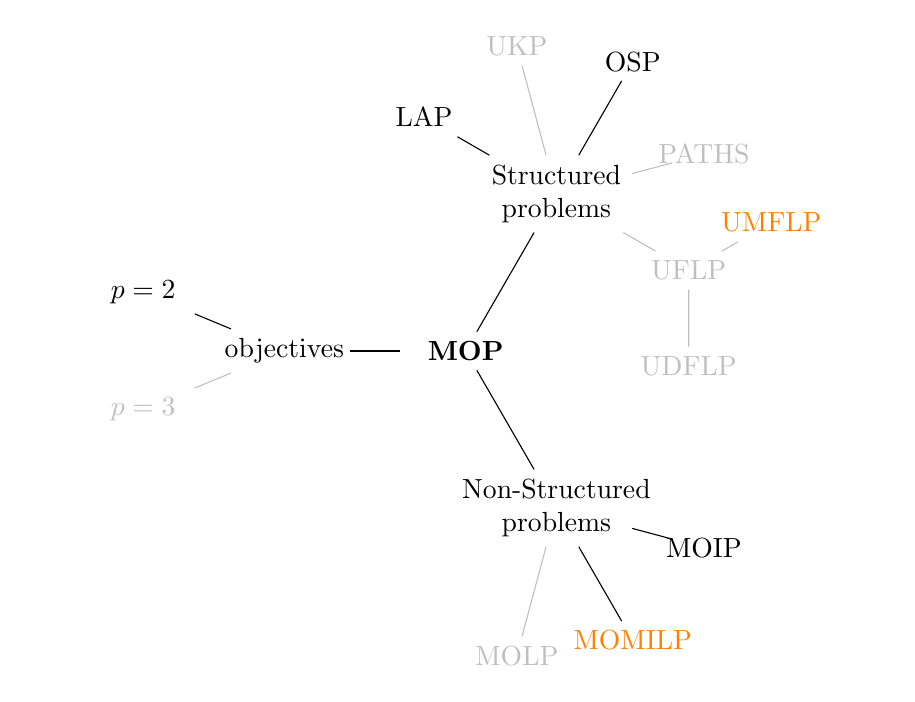
\begin{tikzpicture}[scale=0.485, grow cyclic, text width=2.7cm, align=flush center,
    level 1/.style={level distance=4.75cm,sibling angle=120},
    level 2/.style={level distance=4.0cm,sibling angle=45},
    level 3/.style={level distance=2.5cm,sibling angle=120}]
\node{\normalsize{\textbf{MOP}}}
   child [color=white]{ }
   child { node {Non-Structured\\ problems}
        child [color = black!25]{ node {MOLP}}
        child { node {\orange{MOMILP}}}
        child { node {MOIP}}
    }
    child { node {Structured\\ problems}
        child [color = black!25]{ node {UFLP} 
          child { node {UDFLP}}
          child { node {\orange{UMFLP}}}
          }
        child [color = black!25]{ node {PATHS}}
        child [color = black]{ node {OSP}}
        child [color = black!25]{ node {UKP}}        
        child { node {LAP}}
    }
    child { node {objectives}
        child { node {$p=2$}}
        child [color = black!25]{ node {$p=3$}}
%        child [concept color=green!40]{ node {Themes and Handouts}}
    };


\end{tikzpicture}
\bigskip

\vspace{-15mm}{\orange{Framework of the\\ ANR/DFG research project}}
}

\end{frame}

%
% ================================================================
% 
\begin{frame}{Solutions reached}

For a given problem, the aim is to compute
\vspace{5mm}

\centerline{\textbf{$\mathbf{Y_N}$, the set of nondominated ``points''}}
\vspace{5mm}

corresponding to
\vspace{5mm}

\centerline{\textbf{$\mathbf{X_E}$, a complete set of efficient solutions}}
\vspace{10mm}

More on definitions and notations, refer to this book:

\begin{itemize}
%  \item
  \item[] Matthias Ehrgott.\\ \textit{Multicriteria Optimization.}\\ Springer-Verlag New York, 2005.
\end{itemize}

\end{frame}
    
%
% ================================================================
% 
\begin{frame}{Design of {vOptSolver}}

\hspace{-18mm}
%\begin{center}
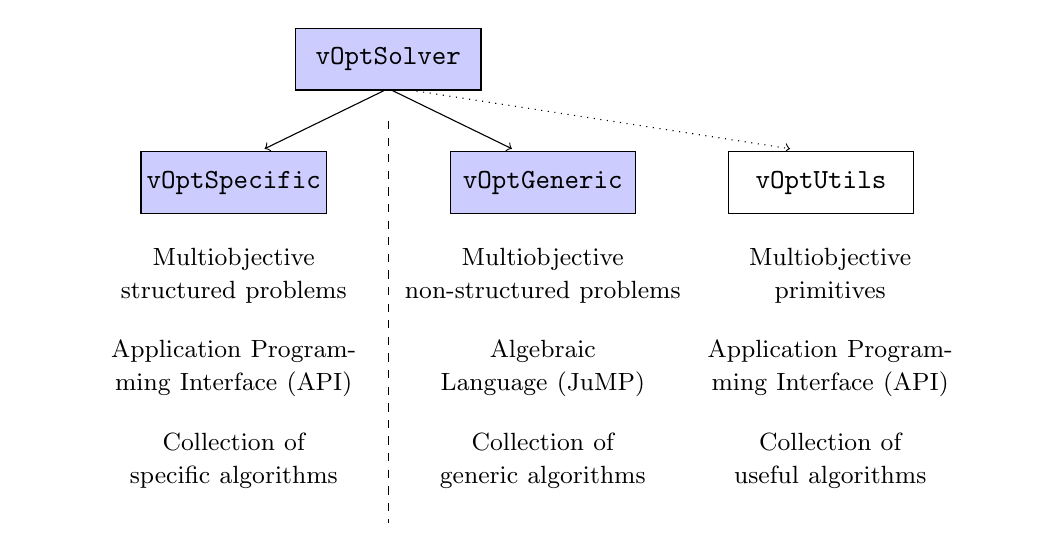
\begin{tikzpicture}[scale=0.785]%[auto]

\draw [fill=blue!20] (4,12) rectangle (7,13);
\node [text width=8cm,text centered] at (5.5,12.5) {\texttt{vOptSolver}};

\draw [->] (5.45,12) -- (3.5,11.05);
\draw [->] (5.55,12) -- (7.5,11.05);
\draw [->, dotted] (5.85,12) -- (12,11.05);

\draw [fill=blue!20] (1.5,10) rectangle (4.5,11);
\node [text width=5cm,text centered] at (3,10.5) {\texttt{vOptSpecific}};
\draw [fill=blue!20] (6.5,10) rectangle (9.5,11);
\node [text width=5cm,text centered] at (8,10.5) {\texttt{vOptGeneric}};
\draw [fill=white!20] (11,10) rectangle (14,11);
\node [text width=5cm,text centered] at (12.5,10.5) {\texttt{vOptUtils}};

\draw  [dashed](5.5,11.5) -- (5.5,5);

\node [text width=4cm,text centered] at (3,9) {\small Multiobjective \\ structured problems};
\node [text width=4cm,text centered] at (3,7.5) {\small Application Programming Interface (API)};
\node [text width=4cm,text centered] at (3,6) {\small {Collection of \\ specific algorithms}};
%\node [text width=4cm,text centered, color=Gray] at (3,4.5) {\footnotesize \texttt{Pkg.Add(vOptSpecific.jl)}};

\node [text width=4cm,text centered] at (8,9) {\small Multiobjective \\ non-structured problems};
\node [text width=4cm,text centered] at (8,7.5) {\small Algebraic\\ Language (JuMP)};
\node [text width=4cm,text centered] at (8,6) {\small {Collection of \\ generic algorithms}};
%\node [text width=4cm,text centered, color=Gray] at (8,4.5) {\footnotesize \texttt{Pkg.Add(vOptGeneric.jl)}};

\node [text width=4cm,text centered] at (12.65,9) {\small Multiobjective \\ primitives};
\node [text width=4cm,text centered] at (12.65,7.5) {\small Application Programming Interface (API)};
\node [text width=4cm,text centered] at (12.65,6) {\small {Collection of \\ useful algorithms}};
%\node [text width=4cm,text centered, color=Gray] at (12.65,4.5) {\footnotesize \texttt{Pkg.Add(vOptUtils.jl)}};

\end{tikzpicture}
%\end{center}

\end{frame}

%
% ================================================================
% 
\begin{frame}{Design of {vOptSolver} in details}

\vspace{-2mm}
%\begin{center}
\hspace{-5mm}
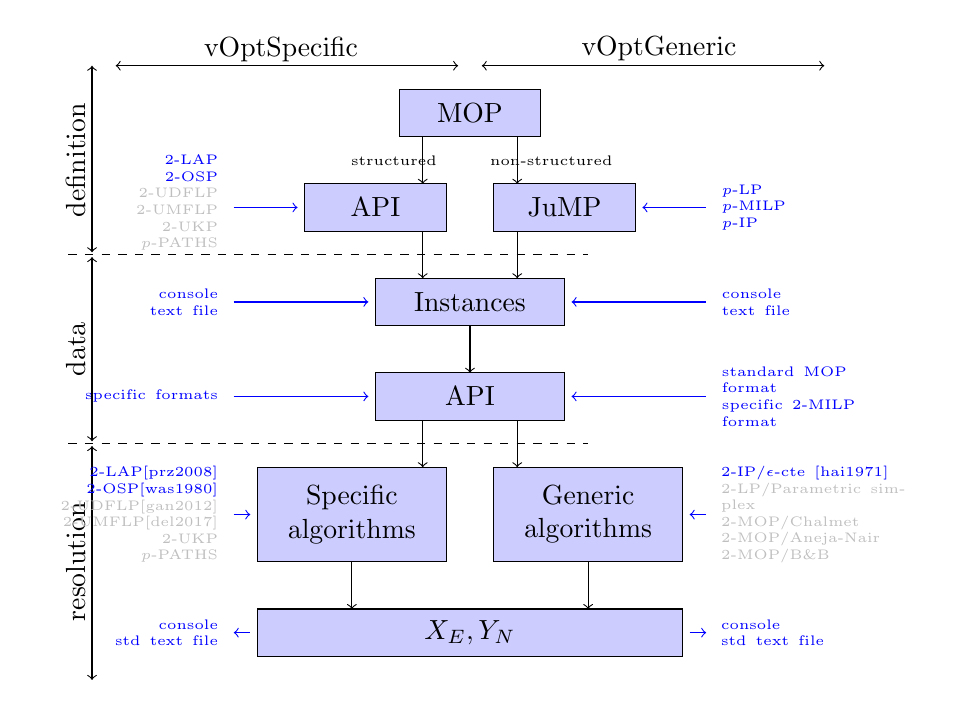
\begin{tikzpicture}[scale=0.6]%[auto]

\draw  [<->](1,13.5) -- (8.25,13.5);
\node [text width=2cm,text centered] at (4.5,13.85) {{vOptSpecific}};
\draw  [<->](8.75,13.5) -- (16,13.5);
\node [text width=2cm,text centered] at (12.5,13.85) {{vOptGeneric}};

\draw [fill=blue!20] (7,12) rectangle (10,13);
\node [text width=8cm,text centered] at (8.5,12.5) {{MOP}};

\draw [->] (7.5,12) -- (7.5,11);
\node [text width=2cm,align=left] at (7.65,11.5) {\tiny{structured}};
\draw [->] (9.5,12) -- (9.5,11);
\node [text width=2cm,align=right] at (9.85,11.5) {\tiny{non-structured}};

\draw [fill=blue!20] (5,10) rectangle (8,11);
\node [text width=8cm,text centered] at (6.5,10.5) {{API}};

\draw [->, color=blue] (3.5,10.5) -- (4.85,10.5);
\node [text width=2cm,align=right, color=blue] at (1.5,10.6) {
{\tiny 2-LAP \\ {2-OSP} \\ \grey{2-UDFLP} \\ \grey{2-UMFLP} \\ \grey{2-UKP} \\ \grey{$p$-PATHS} \\}
};

\draw [fill=blue!20] (9,10) rectangle (12,11);
\node [text width=8cm,text centered] at (10.5,10.5) {{JuMP}};

\draw [<-, color=blue] (12.15,10.5) -- (13.5,10.5);
\node [text width=2cm,align=left, color=blue] at (15.5,10.5) {
{\tiny $p$-LP \\ $p$-MILP \\ $p$-IP \\}
};

\draw [->] (7.5,10) -- (7.5,9);
\draw [->] (9.5,10) -- (9.5,9);

\draw  [dashed](0,9.5) -- (11,9.5);
\draw  [<->](0.5,13.5) -- (0.5,9.55);
\node [text width=2cm,text centered,rotate=90] at (0.15,11.5) {{definition}};

\draw [->, color=blue] (3.5,8.5) -- (6.35,8.5);
\node [text width=2cm,align=right, color=blue] at (1.5,8.5) {
{\tiny console\\ text file\\}
};

\draw [<-, color=blue] (10.65,8.5) -- (13.5,8.5);
\node [text width=2cm,align=left, color=blue] at (15.5,8.5) {
{\tiny console\\ text file\\}
};

\draw [fill=blue!20] (6.5,8) rectangle (10.5,9);
\node [text width=8cm,text centered] at (8.5,8.5) {{Instances}};
\draw [->] (8.5,8) -- (8.5,7);

\draw [->, color=blue] (3.5,6.5) -- (6.35,6.5);
\node [text width=2cm,align=right, color=blue] at (1.5,6.5) {
{\tiny specific formats}
};

\draw [<-, color=blue] (10.65,6.5) -- (13.5,6.5);
\node [text width=2cm,align=left, color=blue] at (15.5,6.5) {
{\tiny standard MOP format\\ specific 2-MILP format\\}
};

\draw [fill=blue!20] (6.5,6) rectangle (10.5,7);
\node [text width=8cm,text centered] at (8.5,6.5) {{API}};

\draw [->] (7.5,6) -- (7.5,5);
\draw [->] (9.5,6) -- (9.5,5);

\draw  [<->](0.5,9.45) -- (0.5,5.55);
\node [text width=2cm,text centered,rotate=90] at (0.15,7.5) {{data}};
\draw  [dashed](0,5.5) -- (11,5.5);
\draw  [<->](0.5,0.5) -- (0.5,5.45);
\node [text width=2cm,text centered,rotate=90] at (0.15,3) {{resolution}};

\draw [->, color=blue] (3.5,4) -- (3.85,4);
\node [text width=2cm,align=right, color=blue] at (1.5,4) {
{\tiny 2-LAP[prz2008] \\ {2-OSP[was1980]} \\ \grey{2-UDFLP[gan2012]} \\ \grey{2-UMFLP[del2017]} \\ \grey{2-UKP} \\ \grey{$p$-PATHS} \\}
};

\draw [fill=blue!20] (4,3) rectangle (8,5);
\node [text width=8cm,text centered] at (6,4) {{Specific\\ algorithms}};

\draw [<-, color=blue] (13.15,4) -- (13.5,4);
\node [text width=2.5cm,align=left, color=blue] at (15.9,4) {
{\tiny 2-IP/$\epsilon$-cte  [hai1971]\\ \grey{2-LP/Parametric simplex} \\ \grey{2-MOP/Chalmet} \\ \grey{2-MOP/Aneja-Nair} \\ \grey{2-MOP/B\&B}\\}
};

\draw [fill=blue!20] (9,3) rectangle (13,5);
\node [text width=8cm,text centered] at (11,4) {{Generic\\ algorithms}};

\draw [->] (6,3) -- (6,2);
\draw [->] (11,3) -- (11,2);

\draw [fill=blue!20] (4,1) rectangle (13,2);
\node [text width=8cm,text centered] at (8.5,1.5) {{$X_E, Y_N$}};

\draw [<-, color=blue] (3.5,1.5) -- (3.85,1.5);
\node [text width=2cm,align=right, color=blue] at (1.5,1.5) {
{\tiny console\\ std text file\\}};

\draw [->, color=blue] (13.15,1.5) -- (13.5,1.5);
\node [text width=2.5cm,align=left, color=blue] at (15.9,1.5) {
{\tiny console\\ std text file\\}
};
\end{tikzpicture}

\end{frame}

%
% ================================================================
% 
\begin{frame}{Design of {vOptSolver} in details}

\texttt{vOptUtils}:\\
\bigskip
 a collection of algorithms for managing and analyzing outcome set
 \bigskip 

\begin{itemize}
  \item multidimensional datastructure for filtering and storing $Y_N$
  \item \grey{primitives for ploting $Y_N$} 
  \item \grey{primitives for analyzing $Y_N$}
\end{itemize}  

\end{frame}

%
% ================================================================
% 
\begin{frame}{Integrated specific algorithms (1/2)}

{\small
\begin{itemize}
\item 2-LAP [prz2008]; in C:\vspace{1mm}\\
         {\tiny A. Przybylski, X. Gandibleux, and M. Ehrgott. Two phase algorithms for the bi-objective assignment problem.
         \textit{European Journal of Operational Research},185(2):509--533, 2008.\\}
         output: $X_E \subseteq \mN^n$, $Y_N \subseteq \Z^p$
         \medskip

\item {2-OSP with here $1\mid . \mid (\Sigma C_i,T_{max})$  [was1980]; in Julia:\vspace{1mm}\\
         {\tiny L.N. Van Wassenhove and L.F. Gelders. Solving a bicriterion scheduling problem. 
         \textit{European Journal of Operational Research}, 4(1):42--48, 1980.\\}
         output: $X_E \subseteq \mN^n$, $Y_N \subseteq \Z^p$
         }
         \medskip
         
\item \grey{ 2-UKP [jor2010]; in Julia:\vspace{1mm}\\
         {\tiny J. Jorge. \textit{Nouvelles propositions pour la résolution exacte du sac à dos multi-objectif unidimensionnel en variables binaires}.
         Th\`ese de doctorat, Université de Nantes - France. 2010.\\}
         output: $X_E \subseteq \mB^n$, $Y_N \subseteq \Z^p$
         }
         \medskip
                  
%\item \grey{ 2-UDFLP [gan2012]; in C++:\vspace{1mm}\\
%         {\tiny X. Gandibleux, A. Przybylski, S. Bourougaa, A. Derrien, A. Grimault: 
%         Computing the efficient frontier for the6480/1 biobjective uncapacitated facility location problem,  2012. 
%         10th International Conference on Multiple649Objective Programming and Goal Programming. June 11-13 2012, Niagara Falls, Canada.\\}
%         output: $X_E \subseteq \mB^n$, $Y_N \subseteq \Z^p$
%         }
%         \smallskip
%         
%\item \grey{ 2-UMFLP [del2017]; in C++:\vspace{1mm}\\      
%         {\tiny Q. Delmée, X. Gandibleux, A. Przybylski. Résolution exacte du problème de localisation de services bi-objectif sans contrainte de capacité en variables mixtes
%ROADEF2017 : 18ème congrès annuel de la Société Française de Recherche Opérationnelle et d'Aide à la Décision, Feb 2017, Metz, France. 2017\\}
%         output: $X_E  \subseteq \mB^{n_1} \times \R^{n_2}$, $Y_N$
%         }
%         
%\item \grey{ PATHS [gan2004]; in C:\vspace{1mm}\\      
%         {\tiny X. Gandibleux, Fr. Beugnies and S. Randriamasy:
%         Martins' algorithm revisited for multi-objective shortest path problems with a MaxMin cost function.
%         4OR: A Quarterly Journal of Operations Research, Volume 4, Number 1, pp. 47-59, 2006. \\}
%         output: $X_E$, $Y_N$
%         }
                  
\end{itemize}
}
\end{frame}

%
% ================================================================
% 
\begin{frame}{Integrated specific algorithms (2/2)}

{\small
\begin{itemize}
%\item 2-LAP [prz2008]; in C:\vspace{1mm}\\
%         {\tiny A. Przybylski, X. Gandibleux, and M. Ehrgott. Two phase algorithmsfor the bi-objective assignment problem.
%         European Journal of Operational Research,185(2):509--533, 2008.\\}
%         output: $X_E \subseteq \mN^n$, $Y_N \subseteq \Z^p$
%         \smallskip
%
%\item 2-OSP with here $1\mid . \mid (\Sigma C_i,T_{max})$  [was1980]; in Julia:\vspace{1mm}\\
%         {\tiny L.N. Van Wassenhove and L.F. Gelders. Solving a bicriterion scheduling problem. 
%         European Journal of Operational Research, 4(1):42--48, 1980.\\}
%         output: $X_E \subseteq \mN^n$, $Y_N \subseteq \Z^p$
%         \smallskip
%         
%\item \grey{ 2-UKP [jor2010]; in Julia:\vspace{1mm}\\
%         {\tiny J. Jorge. Nouvelles propositions pour la résolution exacte du sac à dos multi-objectif unidimensionnel en variables binaires.
%         Th\`ese de doctorat, Université de Nantes - France. 2010.\\}
%         output: $X_E \subseteq \mB^n$, $Y_N \subseteq \Z^p$
%         }
%         \smallskip
%                  
\item \grey{ 2-UDFLP [gan2012]; in C++:\vspace{1mm}\\
         {\tiny X. Gandibleux, A. Przybylski, S. Bourougaa, A. Derrien, A. Grimault.
         Computing the efficient frontier for the 0/1 biobjective uncapacitated facility location problem.
         \textit{10th International Conference on Multiple Objective Programming and Goal Programming}.
         June 11-13 2012, Niagara Falls, Canada.\\}
         output: $X_E \subseteq \mB^n$, $Y_N \subseteq \Z^p$
         }
         \medskip
         
\item \grey{ 2-UMFLP [del2017]; in C++:\vspace{1mm}\\      
         {\tiny Q. Delmée, X. Gandibleux, A. Przybylski. Résolution exacte du problème de localisation de services bi-objectif sans contrainte de capacité en variables mixtes.
         \textit{ROADEF2017 : 18ème congrès annuel de la Société Française de Recherche Opérationnelle et d'Aide à la Décision}, Feb 2017, Metz, France. 2017\\}
         output: $X_E  \subseteq \mB^{n_1} \times \R^{n_2}$, $Y_N$
         }
         \medskip
         
\item \grey{ PATHS [gan2004]; in C:\vspace{1mm}\\      
         {\tiny X. Gandibleux, Fr. Beugnies and S. Randriamasy:
         Martins' algorithm revisited for multi-objective shortest path problems with a MaxMin cost function.
         \textit{4OR: A Quarterly Journal of Operations Research}.
         Volume 4, Number 1, pp. 47-59, 2006. \\}
         output: $X_E$, $Y_N$
         }
                  
\end{itemize}
}
\end{frame}

%
% ================================================================
% 
\begin{frame}{Integrated generic algorithms (1/2)}

{\small
\begin{itemize}
\item 2-IP/$\epsilon$-constraint method [hai1971]; in Julia:\vspace{1mm}\\
         {\tiny Y.V. Haimes, L.S. Lasdon, D.A. Wismer: On a bicriterion formation of the problems of integrated system identification and system optimization. 
         \textit{IEEE Transactions on Systems, Man and Cybernetics}.
         Volume SMC-1, Issue 3, Pages 296-297, July 1971.\\}
         output: $X_E \subseteq \Z^n$, $Y_N \subseteq \Z^p$
         \medskip
     
\item \grey{
         2-IP/dichotomic method:\vspace{1mm}\\   
         {\tiny Aneja, Y. and K. Nair:
          Bicriteria transportation problem. 
          \textit{Management Science} 25 (1), 73?78. 1979.\\}
         output: $X_{SE} \subseteq \Z^n$, $Y_{SN} \subseteq \Z^p$
         }
         \medskip
\item \grey{
         2-IP/Chalmet \& al., 1986:\vspace{1mm}\\   
         {\tiny L.G. Chalmet, L. Lemonidis, and D.J. Elzinga. An algorithm for the bi-criterion integer programming problem. 
         \textit{European Journal of Operational Research}, 25:292-300, 1986.\\}
         output: $X_E \subseteq \Z^n$, $Y_N \subseteq \Z^p$
         }         
%         \medskip
%\item \grey{
%         2-MILP/Vincent \& al., 2014:\vspace{1mm}\\   
%         {\tiny  Th. Vincent, F. Seipp, S. Ruzika, A. Przybylski, X. Gandibleux.
%          Multiple objective branch and bound for mixed 0-1 linear programming: Corrections and improvements for the biobjective case. 
%          \textit{Computers \& Operations Research}, Volume 40, Issue 1, pp. 498--509, 2013.\\
%          Fl. Lucas. \textit{Multiobjective branch \& cut}. Master Thesis, University of Nantes, France. June 2017.\\
%          }
%         output: $X_E \subseteq \Z^n$, $Y_N \subseteq \Z^p$
%         }         
%         \medskip
%         
%\item \grey{
%         2-LP/parametric simplex:\vspace{1mm}\\   
%         {\tiny Description available in: Matthias Ehrgott. \textit{Multicriteria Optimization.} Springer-Verlag New York, 2005.\\}
%         output: $X_{SE} \subseteq \R^n$, $Y_{SN} \subseteq \R^p$
%         }         
\end{itemize}
}
\end{frame}

%
% ================================================================
% 
\begin{frame}{Integrated generic algorithms (2/2)}

{\small
\begin{itemize}
%\item 2-IP/$\epsilon$-constraint method [hai1971]; in Julia:\vspace{1mm}\\
%         {\tiny Y.V. Haimes, L.S. Lasdon, D.A. Wismer: On a bicriterion formation of the problems of integrated system identification and system optimization. 
%         \textit{IEEE Transactions on Systems, Man and Cybernetics}.
%         Volume SMC-1, Issue 3, Pages 296-297, July 1971.\\}
%         output: $X_E \subseteq \Z^n$, $Y_N \subseteq \Z^p$
%         \medskip
%     
%\item \grey{
%         2-IP/dichotomic method:\vspace{1mm}\\   
%         {\tiny Aneja, Y. and K. Nair:
%          Bicriteria transportation problem. 
%          \textit{Management Science} 25 (1), 73?78. 1979.\\}
%         output: $X_{SE} \subseteq \Z^n$, $Y_{SN} \subseteq \Z^p$
%         }
%         \medskip
%\item \grey{
%         2-IP/Chalmet \& al., 1986:\vspace{1mm}\\   
%         {\tiny L.G. Chalmet, L. Lemonidis, and D.J. Elzinga. An algorithm for the bi-criterion integer programming problem. 
%         \textit{European Journal of Operational Research}, 25:292-300, 1986.\\}
%         output: $X_E \subseteq \Z^n$, $Y_N \subseteq \Z^p$
%         }         
%         \medskip
\item \grey{
         2-MILP/Vincent \& al., 2014:\vspace{1mm}\\   
         {\tiny  Th. Vincent, F. Seipp, S. Ruzika, A. Przybylski, X. Gandibleux.
          Multiple objective branch and bound for mixed 0-1 linear programming: Corrections and improvements for the biobjective case. 
          \textit{Computers \& Operations Research}, Volume 40, Issue 1, pp. 498--509, 2013.\smallskip\\
          Fl. Lucas. \textit{Multiobjective branch \& cut}. Master Thesis, University of Nantes, France. June 2017.\\
          }
         output: $X_E \subseteq \mR^{n_1} \times \mZ^{n_2}$, $Y_N $
         }         
         \medskip
         
\item \grey{
         2-LP/parametric simplex:\vspace{1mm}\\   
         {\tiny Description available in: Matthias Ehrgott. \textit{Multicriteria Optimization.} Springer-Verlag New York, 2005.\\}
         output: $X_{SE} \subseteq \R^n$, $Y_{SN} \subseteq \R^p$
         }         
\end{itemize}
}
\end{frame}

%
% ================================================================
% 
\begin{frame}{Selectable (MI)LP Engines}

          \begin{itemize}
            \item   open source:\\   - GLPK (GNU Linear Programming Kit) %\\
            %-  Clp (Coin-or linear programming)
            \medskip
            
            \item   commercial: \\  - CPLEX \\
            - GUROBI
          \end{itemize}  

\vspace{10mm}
NB: CPLEX and GUROBI are currently not available on JuliaBox
\end{frame}

%
% ================================================================
% 
\begin{frame}

\begin{center}
{\Large
 \textcolor[RGB]{52,57,176}{
   Instructions \\ for \\ installing and running vOptSolver \\
 }
} 
\end{center}
\end{frame}

%
% ================================================================
% 
\begin{frame}{Instructions for installing vOptSolver}

vOptSolver has been tested with:
\begin{itemize}
\item Julia v0.6
\item GLPK v4.62
\end{itemize}
\bigskip

Choose between:\\ 
\begin{enumerate}
\item a local use   \\
    \quad - on macOS (tested on v10.12.5) \\
    \quad  - on linux (tested on ubuntu 14.04 LTS) \\
    \quad  - on windows (perhaps later...)
\medskip
\item a distant use \\
     \quad - in the cloud with JuliaBox.
\end{enumerate}


\end{frame}

%
% ================================================================
% 
\begin{frame}{Instructions for a distant use in the cloud}

\begin{itemize}
\item Local installation
\begin{enumerate}
  \item nothing to do
\end{enumerate}
\medskip
  
\item Run Julia
\begin{enumerate}
  \item go to \url{https://juliabox.com} and sign in to open a session
  \item click on the icon ``console''
  \item when the prompt is ready, type in the console \\
      \green{\texttt{julia}}
\end{enumerate}
\medskip

\item Before the first use of \texttt{vOptSolver}, add the following packages:
\begin{enumerate}
  \item when the prompt \textit{julia} is ready, type in the terminal \\ 
     \green{\texttt{Pkg.add("{GLPK}"); Pkg.add("GLPKMathProgInterface")}}  
     \green{\texttt{Pkg.clone("\url{http://github.com/vOptSolver/vOptGeneric.jl}")}}\\
     \green{\texttt{Pkg.clone("{http://github.com/vOptSolver/vOptSpecific.jl}")}}
     \green{\texttt{Pkg.build("{vOptSpecific}")}}     
\end{enumerate}  
At this point, vOptSolver is properly installed
\medskip

%\item ``vOptSolver'' is ready !
\end{itemize}

\end{frame}

%
% ================================================================
% 
\begin{frame}{Instructions for a local use on your own computer}

\begin{itemize}
\item Local installation
\begin{enumerate}
  \item install Julia on your computer, instructions here:\\
  \quad \url{http://julialang.org/downloads/}
  \item install (e.g.) GLPK on your computer, instructions here:\\
  \quad \url{http://jump.readthedocs.io/en/latest/installation.html}  
  \item[] \hspace{-4mm}NB: a standard C/C++ compiler must be installed (GCC is suggested)
\end{enumerate}
\smallskip
At this point, Julia and GLPK are properly installed\medskip
  
\item Run Julia
\begin{enumerate}
  \item on linux: open a console on your computer;  when the prompt is ready, type in the console      \green{\texttt{julia}}
  \item on macOS: locate the application julia and click on the icon; julia console comes on the screen
\end{enumerate}
\medskip

\item Before the first use of \texttt{vOptSolver}, add both following packages:
\begin{enumerate}
  \item when the prompt {julia} is ready, type in the console \\ 
     \green{\texttt{Pkg.add("{GLPK}"); Pkg.add("GLPKMathProgInterface")}}    
     \green{\texttt{Pkg.clone("\url{http://github.com/vOptSolver/vOptGeneric.jl}")}}\\
     \green{\texttt{Pkg.clone("{http://github.com/vOptSolver/vOptSpecific.jl}")}}
     \green{\texttt{Pkg.build("{vOptSpecific}")}}         
\end{enumerate}  
\smallskip
At this point, vOptSolver is properly installed
%\item ``vOptSolver'' is ready !
\end{itemize}

\end{frame}

%
% ================================================================
% 
\begin{frame}{Instructions for running vOptSolver}

When vOptSolver is properly installed, vOptSpecific and vOptGeneric are ready locally or in the cloud.
\medskip

\begin{itemize}
  
\item Run Julia
\begin{enumerate}
  \item open a console on your computer or in the cloud
  \item when the prompt is ready, type in the console \\
      \green{\texttt{julia}}
\end{enumerate}
  \item when the prompt \textit{julia} is ready, type in the terminal \\ 
    \begin{enumerate}
      \item    \green{\texttt{using vOptSpecific}}
      \item    \green{\texttt{using vOptGeneric}}
      \item    \green{\texttt{using GLPK ; using GLPKMathProgInterface}}            
    \end{enumerate}
    Remark 1: you may invoke only \texttt{using vOptSpecific} if you are only working with  \texttt{vOptSpecific}. Same remark for \texttt{vOptGeneric}.\\
    Remark 2: you may invoke CPLEX or GUROBI in the place of GLPK (ps: in local mode, the MILP solver selected must be properly installed)    
\medskip

\item vOptSpecific and vOptGeneric are ready. See examples for further informations

\medskip

%\item ``vOptSolver'' is ready !
\end{itemize}


\end{frame}

%
% ================================================================
% 
\begin{frame}

\begin{center}
{\Large
 \textcolor[RGB]{52,57,176}{
   vOptSpecific problem by problem\\
   \vspace{5mm}
   {\small
   definition (problem, inputs) \\
   data (console, text file) \\
   resolution (API, outputs, text file) \\
   }
 }
} 
\end{center}
\end{frame}

%%
%% ================================================================
%% 
\input{2lap.tex}

%\begin{frame}{\textbf{LAP} $\mid$ Definition $\mid$ The linear assignment problem}
%
%    
%    \begin{center}
%$
%\quad
%\left [
%\begin{array}{lcllllll}
%
%\ &  \min z^k & =  & \displaystyle{\sum_{i=1}^{n}\sum_{j=1}^{n} c^k_{ij} x_{ij}}  & & k=1,\dots,p\vspace{2mm} \\
%
% & s/c  & &   \displaystyle{\sum_{i=1}^{n}  x_{ij}}   =  1 & \ &  j=1,\dots ,n \  \ \  \\
%  &       & &   \displaystyle{\sum_{j=1}^{n}  x_{ij}}   =  1 & & i=1,\dots ,n \    \vspace{2mm} \\
%
% & & &  x_{ij} = (0,1) &&   i=1,\dots ,n  \vspace{-1mm}\\
% & & &   & & j=1,\dots ,n\\ 
% 
%\end{array}
%\right ]
%$ \hfill (p-LAP)
%\end{center}
%\end{frame}
%
%%
%% ================================================================
%% 
%\begin{frame}{LAP $\mid$ Definition $\mid$ Inputs}
%
%Valid for 2-LAP.
%\bigskip
%
%              \begin{itemize}
%                \item \texttt{n} (integer): \\ number $n$ of assignments task-resource 
%                           \medskip
%                %\item \texttt{p} (integer): \\ number $p$ of objectives, $k=1\dots p$                  
%                \item \texttt{C1} (matrix of $n \times n$ of integers): \\  coefficients $c^1_{ij}$ of the objective 1  
%                           \medskip
%                \item \texttt{C2} (matrix of $n \times n$ of integers): \\  coefficients $c^2_{ij}$ of the objective 2                                         
%              \end{itemize}
%\end{frame}
%
%%
%% ================================================================
%% 
%\begin{frame}[fragile=singleslide]{LAP $\mid$ Data $\mid$ Example (console)}
%
%{\small
%\begin{verbatim}
%n  =  5
%
%C1 = [  3   9   0   0   6 ;
%       16   0   6  12  19 ;
%        2   7  11  15   8 ;
%        4  11   7  16   3 ;
%        2   5   1   9   0   ]
%
%C2 = [ 16   5   6  19  12 ;
%       15   7  13   7   7 ;
%        1   2  13   2   3 ;
%       14   7   8   1   7 ;
%       10  10   1   0   0   ]
%\end{verbatim}
%}
%
%\end{frame}
%
%%
%% ================================================================
%% 
%\begin{frame}[fragile=singleslide]{LAP $\mid$ Data $\mid$ Example (text file)}
%
%\begin{columns}
%\begin{column}{0.3\textwidth}
%{\small
%\begin{verbatim}
%5
% 3   9   0   0   6 
%16   0   6  12  19 
% 2   7  11  15   8 
% 4  11   7  16   3 
% 2   5   1   9   0   
%16   5   6  19  12 
%15   7  13   7   7 
% 1   2  13   2   3 
%14   7   8   1   7 
%10  10   1   0   0 
%\end{verbatim}
%}
%\end{column}
%\begin{column}{0.3\textwidth}
%\vspace{-2mm}
%%\begin{center}
%\hspace{-5mm}
%\begin{tikzpicture}[scale=0.625]%[auto]
%
%\draw  [<->, color=blue](0,-1) -- (0,1.85);
%\draw  [<->, color=blue](0,2.10) -- (0,5.0);
%\draw  [<->, color=blue](0,5.2) -- (0,5.7);
%\node [text width=1cm,align=left, color=blue] at (1.5,5.45) {{\texttt{n}}};
%\node [text width=1cm,align=left, color=blue] at (1.5,3.6) {{\texttt{C1}}};
%\node [text width=1cm,align=left, color=blue] at (1.5,0.5) {{\texttt{C2}}};
%\draw  [-, dotted, color=blue](-1,2) -- (1,2);
%\draw  [-, dotted, color=blue](-1,5.1) -- (1,5.1);
%\end{tikzpicture}
%\vfill
%\end{column}
%\begin{column}{0.15\textwidth}
%
%\end{column}
%\end{columns}
%
%\vspace{10mm}
%\begin{itemize}
%%\item  \blue{createLAP}\\
%%          Create a new instance of a LAP     \\
%%          \texttt{id = createLAP(  ) }
%\item  \blue{load2LAP}\\
%          Load an instance of a 2-LAP from the file \texttt{fname}    \\
%           \texttt{id = \texttt{{load2}LAP( fname ) }} 
%           \medskip
%\end{itemize}
%
%\end{frame}
%
%%
%% ================================================================
%% 
%\begin{frame}{LAP $\mid$ Resolution $\mid$ API}
%
%\begin{itemize}
%%\item  \blue{createLAP}\\
%%          Create a new instance of a LAP     \\
%%          \texttt{id = createLAP(  ) }
%\item  \blue{set2LAP}\\
%          Create a new instance of a 2-LAP and set up all required values    \\
%           \texttt{id = \texttt{{set2}LAP( n , C1, C2 ) }} 
%           \medskip
%%\item  \blue{set2LAP}\\
%%          Set up all required values of a 2-LAP\\
%%          \texttt{set2LAP( id , n , C1, C2 ) } 
%\item  \blue{LAP\_Przybylski2008} \\
%          Set up the solver to use for the 2-LAP\\
%          \texttt{solver = LAP\_Przybylski2008( ) }
%          \medskip
%\item  \blue{solveMOP}\\
%          Solve the instance provided with the mentioned solver and return the results \\
%          \texttt{z1, z2, $\sigma$ = solveMOP( id , solver ) }
%%          \medskip
%%\item  \blue{get\red{2}LAP}\\
%%          Retrieve   \\
%%          \texttt{results = get\red{2}LAP( id ) }         
%\end{itemize}
%
%\end{frame}
%
%%
%% ================================================================
%% 
%\begin{frame}{LAP $\mid$ Resolution $\mid$ Outputs (specification)}
%
%Valid for 2-LAP.
%\bigskip
%
%solveMOP returns:
%\medskip
%                           \begin{itemize}
%                            %  \item $CPUt$: \\ the time consumed
%%                              \item $nYn$: \\ the number of non-dominated points
%                              \item z1: vector of $1\dots \mid Y_N \mid $ of integers
%                              \item z2: vector of $1\dots \mid Y_N \mid $ of integers
%                              \item $\sigma$: vector of $1,\dots, \mid Y_N \mid $ of  ($\sigma_1, \dots, \sigma_n$)
%                                                                                         
%%                              $$ z_1, z_2, \sigma_1, \dots, \sigma_n$$
%                              where
%                               \begin{itemize}
%%                                     \item $z_k, \ k=1,\dots,p$ of integers:  performances 
%                                     \item $\sigma_i (\ i=1,\dots,n$): integer;  a permutation coding ($x_{ij}=1 \Leftrightarrow \sigma_i=j$)
%                                \end{itemize}
%                           \end{itemize}               
%
%\end{frame}
%
%%
%% ================================================================
%% 
%\begin{frame}{LAP $\mid$ Resolution $\mid$ Outputs (text file)}
%\red{a ecrire}
%\end{frame}

%
% ================================================================
% 

\input{2OSP.tex}
%
%\begin{frame}{\textbf{OSP} $\mid$ Definition $\mid$ One machine scheduling problem}
%
%The general one machine scheduling problem considered here is defined as:
%
%$$ \hspace{30mm} 1\mid r_i \mid (f_1,f_2)  \hspace{30mm} \mbox{(2-OSP)}$$
%\medskip 
%
%and the specific OSP  currently considered is:
%
%$$1\mid . \mid (\Sigma C_i,T_{max}) \hspace{12mm}$$
%
%\end{frame}
%
%%
%% ================================================================
%% 
%\begin{frame}{OSP $\mid$ Definition $\mid$ Inputs}
%
%Valid for 2-OSP.
%\bigskip
%              \begin{itemize}
%                \item \texttt{n} (integer): \\ number $n$ of jobs, $i=1\dots n$   
%                                           \medskip
%                \item \texttt{r} (vector of $n$  integers): \\   $r_{i}$,  the release date for job $i$                
%                                           \medskip    
%                \item \texttt{p} (vector of $n$  integers): \\   $p_{i}$, the processing time for job $i$         
%                                           \medskip    
%                \item \texttt{d} (vector of $n$  integers): \\  $d_{i}$, the due date for job $i$     
%                                           \medskip
%                \item \texttt{w} (vector of $n$  integers): \\  $w_{i}$, the weight associated to job $i$                              
%              \end{itemize}
%\end{frame}
%
%%
%% ================================================================
%% 
%\begin{frame}[fragile=singleslide]{OSP $\mid$ Data $\mid$ Example (console)}
%
%{\small
%\begin{verbatim}
%n = 4
%p = [  2   4   3   1 ]
%d = [  1   2   4   6 ]
%r = [  0   0   0   0 ]
%w = [  1   1   1   1 ]
%\end{verbatim}
%}
%
%\end{frame}
%
%%
%% ================================================================
%% 
%\begin{frame}[fragile=singleslide]{OSP $\mid$ Data $\mid$ Example (text file)}
%
%\begin{columns}
%\begin{column}{0.3\textwidth}
%{\small
%\begin{verbatim}
%4
%2   4   3   1 
%1   2   4   6 
%0   0   0   0 
%1   1   1   1 
%\end{verbatim}
%\vspace{1mm}
%}
%\end{column}
%\begin{column}{0.3\textwidth}
%\vspace{-2mm}
%%\begin{center}
%\hspace{-5mm}
%\begin{tikzpicture}[scale=0.45]%[auto]
%
%\draw  [<->, color=blue](0,1.2) -- (0,1.7);
%\draw  [<->, color=blue](0,2.2) -- (0,2.7);
%\draw  [<->, color=blue](0,3.2) -- (0,3.7);
%\draw  [<->, color=blue](0,4.2) -- (0,4.7);
%\draw  [<->, color=blue](0,5.2) -- (0,5.7);
%
%\node [text width=1cm,align=left, color=blue] at (1.5,5.45) {{\texttt{n}}};
%\node [text width=1cm,align=left, color=blue] at (1.5,4.45) {{\texttt{p}}};
%\node [text width=1cm,align=left, color=blue] at (1.5,3.45) {{\texttt{d}}};
%\node [text width=1cm,align=left, color=blue] at (1.5,2.45) {{\texttt{r}}};
%\node [text width=1cm,align=left, color=blue] at (1.5,1.45) {{\texttt{w}}};
%
%\draw  [-, dotted, color=blue](-1,5) -- (1,5);
%\draw  [-, dotted, color=blue](-1,4) -- (1,4);
%\draw  [-, dotted, color=blue](-1,3) -- (1,3);
%\draw  [-, dotted, color=blue](-1,2) -- (1,2);
%\end{tikzpicture}
%\vfill
%\end{column}
%\begin{column}{0.15\textwidth}
%
%\end{column}
%\end{columns}
%
%\vspace{10mm}
%\begin{itemize}
%\item  \red{load2OSP}\\
%          Load an instance of a 2-OSP from the file \texttt{fname}    \\
%           \texttt{id = \texttt{\red{load2OSP}( fname ) }} 
%           \medskip
%\end{itemize}
%
%\end{frame}
%
%%
%% ================================================================
%% 
%\begin{frame}{OSP $\mid$ Resolution $\mid$ API}
%
%\begin{itemize}
%\item  \red{set2OSP}\\
%          Create a new instance of a 2-OSP and set up all required values    \\
%           \texttt{id = \texttt{\red{set2OSP}( n , P, D, R, W ) }} 
%           \medskip
%\item  \red{OSP\_vanwassenhove1980} \\
%          Set up the solver to use for the 2-OSP\\
%          \texttt{solver = OSP\_vanwassenhove1980( ) }
%          \medskip
%\item  \red{solve2OSP}\\
%          Solve an instance of a 2OSP with the mentioned solver and return the results \\
%          \texttt{status = solve\red{2OSP}( id , solver ) }
%          \medskip
%%\item  \red{get2OSP}\\
%%          Retrieve the results  \\
%%          \texttt{results = \red{get2OSP}( id ) }         
%\end{itemize}
%
%\end{frame}
%
%%
%% ================================================================
%% 
%\begin{frame}{OSP $\mid$ Resolution $\mid$ Outputs (specification)}
%
%Valid for 2-OSP.
%\bigskip
%
%Non-dominated parts of the 2-LAP is defined by a set of points:
%\medskip
%                           \begin{itemize}
%                             % \item $CPUt$: \\ the time consumed
%                              \item $nYn$: \\ the number of non-dominated points
%                              \item $Yn$: \\the list of points,  each point is defined by 
%                              $$ z_1, z_2, \sigma_1, \dots, \sigma_n$$
%                              where
%                               \begin{itemize}
%                                     \item $z_k, \ k=1,\dots,p$ of integers:  performances 
%                                     \item $\sigma_i, \ i=1,\dots,n$ of integers:  permutation coding ($\sigma_i=j  \Leftrightarrow \mbox{ job } j \mbox{ in position } i$)
%                                \end{itemize}
%                           \end{itemize}               
%
%\end{frame}
%
%%
%% ================================================================
%% 
%\begin{frame}{OSP $\mid$ Resolution $\mid$ Outputs (text file)}
%\red{a ecrire}
%\end{frame}

%
% ================================================================
% 
\begin{frame}

\begin{center}
{\Large
 \textcolor[RGB]{52,57,176}{
   vOptGeneric problem by problem\\
   \vspace{5mm}
   {\small
   definition (problem, inputs, JuMP) \\
   data (console, text file) \\
   resolution (solve, outputs, text file) \\
   }
 }
} 
\end{center}
\end{frame}

%
% ================================================================
% 


%
% ================================================================
% 
\begin{frame}{MOMILP-MOLP-MOIP $\mid$ Definition}

\hspace{-4mm}
Three Multi Objective Linear Optimization Problems:


\begin{columns}
\begin{column}{0.33\textwidth}
$$
\begin{array}{rcl}
\min z(x) & = & {C}x\\
\hbox{s/t } Tx & \leqq & d\\
x & \in & 
\mR^{n_1} \times \mZ^{n_2}\\
\notag
\end{array}
$$
\begin{center}
Multi Objective Mixed-Integer Linear Problem (MOMILP)
\end{center}
\end{column}
\begin{column}{0.33\textwidth}
$$
\begin{array}{rcl}
\min z(x) & = & {C}x\\
\hbox{s/t } Tx & \leqq & d\\
x & \in & 
\mR^{n_1}\\
\notag
\end{array}
$$
\begin{center}
Multi Objective\\ Linear \\Problem (MOLP)
\end{center}
\end{column}
\begin{column}{0.33\textwidth}
$$
\begin{array}{rcl}
\min z(x) & = & {C}x\\
\hbox{s/t } Tx & \leqq & d\\
x & \in & 
\mZ^{n_2}\\
\notag
\end{array}
$$
\begin{center}
Multi Objective\\ Integer \\Problem (MOIP)
\end{center}
\end{column}
\end{columns}
\medskip

\bigskip
\noindent 
where:
%\vfill
$$
\begin{array}{rcl}
%\only<1-2>{\blue{x \in \mR^{n_1} \times \mZ^{n_2}}
%& \longrightarrow & n=n_1+n_2 \hbox{ variables, } j = 1,\ldots,n\\}
%\only<3>{\blue{x \in \mR^{n_1}}
%& \longrightarrow & n=n_1+n_2 \hbox{ variables, } j = 1,\ldots,n\\}
%\only<4>{\blue{x \in \mZ^{n_2}}
%& \longrightarrow & n=n_1+n_2 \hbox{ variables, } j = 1,\ldots,n\\}
T \in \mZ^{m \times n} & \longrightarrow & m \hbox{ constraints, } i = 1,\ldots,m\\
%
C \in \mZ^{n\times p} & \longrightarrow & \hbox{the objective matrix}\\
%\only<2>{\red {C \in \mZ^{n\times p}} & \red {\longrightarrow} & \hbox{\red {the objective matrix}}\\}
%\only<3->{C \in \mZ^{n\times p} & \longrightarrow & \hbox{the objective matrix}\\}
%
X=\{x \in \mR^{n_1} \times \mZ^{n_2}| Tx\leq d\}\subseteq\mR^n  & \longrightarrow & \hbox{the set of feasible solutions}\\
Y=z(X)\subseteq \mR^p & \longrightarrow & \hbox{the set of images}\\
\notag
\end{array}
$$

\end{frame}

%
% ================================================================
% 
\begin{frame}{MOMILP-MOLP-MOIP $\mid$ Formulation}

Following spectifications of JuMP for formulating a model, see:
\begin{itemize}
  \item \url{http://jump.readthedocs.io/en/latest/quickstart.html\#creating-a-model}
\end{itemize}

\bigskip

Plus:

\begin{itemize}
  \item \texttt{@addobjective( <model>, <opt>, <function>)}\bigskip\\

  where 
  \begin{itemize}
  \item model: id of the model concerned
  \item opt: function to \texttt{Min} imize or \texttt{Max} imize
  \item function: definition of the function
  \end{itemize}
\end{itemize}  

\end{frame}

%
% ================================================================
% 
\begin{frame}[fragile=singleslide]{MOMILP-MOLP-MOIP $\mid$ Example of formulation}

{\small
\begin{columns}
\begin{column}{0.33\textwidth}
$$
\begin{array}{rlcl}
\min          & c^1_1x_1+c^1_2x_2\\
\min          & c^2_1x_1+c^2_2x_2\\
\hbox{s/t } &  t_{11}x_1+t_{12}x_2  \leq  d_1\\
                 &  t_{21}x_1+t_{22}x_2  \leq  d_2\\
                 & x_1  \in \mR, x_2 \in \mZ\\
\notag
\end{array}
$$
%%
$$
\begin{array}{rlcl}
\min          & c^1_1x_1+c^1_2x_2\\
\min          & c^2_1x_1+c^2_2x_2\\
\hbox{s/t } &  t_{11}x_1+t_{12}x_2  \leq  d_1\\
                 &  t_{21}x_1+t_{22}x_2  \leq  d_2\\
                 & x_1, x_2  \in \mR\\
\notag
\end{array}
$$
%%
$$
\begin{array}{rlcl}
\min          & c^1_1x_1+c^1_2x_2\\
\min          & c^2_1x_1+c^2_2x_2\\
\hbox{s/t } &  t_{11}x_1+t_{12}x_2  \leq  d_1\\
                 &  t_{21}x_1+t_{22}x_2  \leq  d_2\\
                 & x_1, x_2 \in \mZ\\
\notag
\end{array}
$$
\end{column}
%%
%%

\begin{column}{0.66\textwidth}

{\scriptsize
\begin{verbatim}
# --- create a MOMILP and set the model ---
  MOMILP = vModel(solver=<working on it>) 
  @variable(MOMILP, x1 >= 0)
  @variable(MOMILP, x2 >= 0, Int)
  @addobjective(MOMILP, Min, c11*x1 + c12*x2)
  @addobjective(MOMILP, Min, c21*x1 + c22*x2)  
  @constraint(MOMILP, t11*x1 + t12*x2 <= d1)
  @constraint(MOMILP, t21*x1 + t22*x2 <= d2)
\end{verbatim}  
}
%%
%%
{\scriptsize
\begin{verbatim}
# --- create a MOLP and set the model ---
  MOLP = vModel(solver=<working on it>) 
  @variable(MOMILP, x1 >= 0)
  @variable(MOMILP, x2 >= 0)
  @addobjective(MOLP, Min, c11*x1 + c12*x2)
  @addobjective(MOLP, Min, c21*x1 + c22*x2)  
  @constraint(MOLP, t11*x1 + t12*x2 <= d1)
  @constraint(MOLP, t21*x1 + t22*x2 <= d2)
\end{verbatim}  
}
%%
%%
{\scriptsize
\begin{verbatim}
# --- create a MOIP and set the model ---
  MOIP = vModel(solver=GLPKSolverMIP()) 
  @variable(MOIP, x1 >= 0, Int)
  @variable(MOIP, x2 >= 0, Int)
  @addobjective(MOIP, Min, c11*x1 + c12*x2)
  @addobjective(MOIP, Min, c21*x1 + c22*x2)  
  @constraint(MOIP, t11*x1 + t12*x2 <= d1)
  @constraint(MOIP, t21*x1 + t22*x2 <= d2)
\end{verbatim}  
}

\end{column}
\end{columns}
}

\end{frame}

%
% ================================================================
% 
\begin{frame}[fragile=singleslide]{MOMILP-MOLP-MOIP  $\mid$ Data $\mid$ Example (console)}

{\small
\begin{verbatim}
c11 =  3   ;  c12 =  1
c21 = -1   ;  c22 = -2

t11 =  0   ;  t12 =  1   ;  d1 = 3
t21 =  3   ;  t22 = -1   ;  d2 = 6
\end{verbatim}
}

\end{frame}

%
% ================================================================
% 
\begin{frame}[fragile=singleslide]{MOMILP-MOLP-MOIP $\mid$ Data $\mid$ Example (format MOP)}

\begin{columns}
\begin{column}{0.3\textwidth}
{\small
%\begin{verbatim}
%\red{a ecrire}
%\end{verbatim}
}
\end{column}
\begin{column}{0.3\textwidth}
%\red{a ecrire}
\end{column}
\begin{column}{0.15\textwidth}
\end{column}
\end{columns}

\vspace{5mm}
%\begin{itemize}
%\item  
\blue{parseMOP}\\
          Load an instance (MOP format) from the file \texttt{fname}    \\
           \texttt{jumpModel  = \texttt{{parseMOP}( fname , solver=<solver to invoke> ) }} 
           \medskip
%\end{itemize}

\blue{writeMOP}\\
  Write a model according to the MOP format to a file \texttt{fname} \\
           \texttt{{writeMOP}( vModel , fname )}  

\vspace{5mm}
NB: the MOP format is an extension of \\
\smallskip
\quad the MPS format\\ \qquad (\url{https://en.wikipedia.org/wiki/MPS_(format)})\\
\smallskip
\quad  to multiple objectives\\ \qquad (\url{http://moplib.zib.de/format_desc/mop_format.pdf})
\end{frame}

%
% ================================================================
% 
\begin{frame}[fragile=singleslide]{MOMILP-MOLP-MOIP $\mid$ Example of resolution}

{\small
\begin{columns}
\begin{column}{0.33\textwidth}
MOMILP\\
{\scriptsize
Algorithm: branch\&bound\\
Solver: \grey{working on it}\\
}
\vspace{15mm}
%%
MOLP\\
{\scriptsize
Algorithm: parametric simplex\\
Solver: \grey{working on it}\\
}
\vspace{15mm}
%%
MOIP\\
{\scriptsize
Algorithm: $\epsilon$-constraint\\
Solver: GLPK or CPLEX\\
}
%\vspace{3mm}
\end{column}
%%
%%

\begin{column}{0.66\textwidth}
{\scriptsize
\begin{verbatim}  
# --- solve the model ---
  status = solve( MOMILP )
  
# --- Print the results ---
  print_X_E( MOMILP )
\end{verbatim}
}
\vspace{5mm}
%%
%%
{\scriptsize
\begin{verbatim}  
# --- solve the model ---
  status = solve( MOLP )

# --- Print the results ---
  print_X_E( MOLP )
\end{verbatim}
}
\vspace{5mm}
%%
%%
{\scriptsize
\begin{verbatim}  
# --- solve the model ---
  status = solve( MOIP , method =:epsilon , step = 0.5 )
  
# --- Print the results ---
  print_X_E( MOIP )
  
# --- Get the results ---
  getY_N( MOIP )  
\end{verbatim}
}

\end{column}
\end{columns}
}

\end{frame}

%
% ================================================================
% 
\begin{frame}{MOMILP-MOLP-MOIP $\mid$ Resolution $\mid$ Outputs (specification)}

$Y_N$ of the 2-MOP is defined by 
\begin{itemize}
  \item \grey{2-MILP: a mixed nondominated set (composed of edges that are either closed, half-open, open or reduced to a point)}
  \item \grey{2-LP: a continuous nondominated set (composed of edges)}
  \item 2-IP: a discrete nondominated set (composed of points)
\end{itemize}  

%with respect to this format:
%
%\medskip
%                           \begin{itemize}
%                              \item $CPUt$: \\ the time consumed\\
%                              \red{a ecrire}
%%                              \item $nYn$: \\ the number of non-dominated points
%%                              \item $Yn$: \\the list of points,  each point is defined by 
%%                              $$ z_1, z_2, \sigma_1, \dots, \sigma_n$$
%%                              where
%%                               \begin{itemize}
%%                                     \item $z_k, \ k=1,\dots,p$ of integers:  performances 
%%                                     \item $\sigma_i, \ i=1,\dots,n$ of integers:  permutation coding ($x_{ij}=1 \Leftrightarrow \sigma_i=j$)
%%                                \end{itemize}
%                           \end{itemize}               

\end{frame}

%
% ================================================================
% 
%\begin{frame}{MOMILP-MOLP-MOIP $\mid$ Resolution $\mid$ Outputs (text file)}
%\red{a ecrire}
%\end{frame}

%
% ================================================================
% 
\begin{frame}

\begin{center}
{\Large
 \textcolor[RGB]{52,57,176}{
   Technical overview
 }
} 
\end{center}
\end{frame}

%
% ================================================================
% 
\begin{frame}{Technical overview ${\blue{.}} {\red{.}} {\green{.}} \magenta{.}$}

\vspace{5mm}
%\begin{center}
\hspace{-0mm}
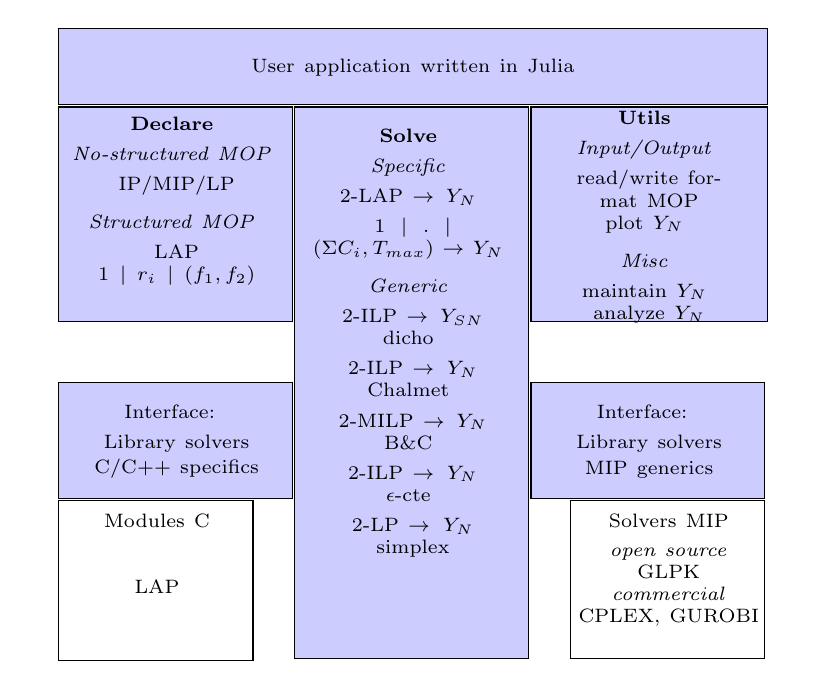
\begin{tikzpicture}[auto]

%\node  at (2.47,3.9) {\scriptsize{MOLP}};
%\node  at (2.5,3.65) {\scriptsize{MOCO}};
%\node  at (2.44,3.4) {\scriptsize{MOIP}};
%\node  [color=orange] at (2.61,3.15) {\scriptsize{MOMILP}};
%
%\matrix [matrix anchor=west, right delimiter=\}] at (2.75,3.45)
%{
%\node { };\\
%\node { }; \\
%\node { }; \\
%};

\draw [fill=blue!20] (1,5+0.03) rectangle (10,6); % julia
\node [text width=8cm,text centered] at (5.5,5.5) {\scriptsize{User application written in Julia}};
%
\draw [fill=blue!20, ] (1,2.25+0.03) rectangle (4-0.03,5); 
\node [text width=3cm,text centered] at (2.5,3.8)  {\scriptsize{\textbf{Declare}  \vspace{1mm}\\ 
\textit{No-structured MOP}  \vspace{1mm}\\
 IP/MIP/LP\vspace{2mm}\\
\textit{Structured MOP} \vspace{1mm}\\
LAP \\ $1\mid r_i \mid (f_1, f_2)$ \\ }};
%
\draw [fill=blue!20, ] (4,-2.0) rectangle (7-0.03,5); 
\node [text width=3cm,text centered] at (5.5,2){\scriptsize{\textbf{Solve}  \vspace{1mm}\\
\textit{Specific}  \vspace{1mm}\\
2-LAP $\rightarrow Y_{N}$ \vspace{1mm}\\ 
$1\mid . \mid (\Sigma C_i,T_{max}) \rightarrow Y_{N}$}  \vspace{2mm}\\
\textit{Generic} \vspace{1mm}\\
2-ILP $\rightarrow Y_{SN}$\\  dicho  \vspace{1mm}\\
2-ILP $\rightarrow Y_{N}$\\  Chalmet  \vspace{1mm}\\
2-MILP $\rightarrow Y_{N}$\\  B\&C  \vspace{1mm}\\
2-ILP $\rightarrow Y_{N}$\\ $\epsilon$-cte  \vspace{1mm}\\
2-LP $\rightarrow Y_{N}$\\ simplex  \\
};

%
\draw [fill=blue!20, ] (7,2.25+0.03) rectangle (10,5); 
%\draw (7,0.03) rectangle (10,2); 
%\draw[dashed,thin] (7,2.5) -- (10,2.5);
\node [text width=3cm,text centered] at (8.5,3.6) {\scriptsize{\textbf{Utils}  \vspace{1mm}\\ 
\textit{Input/Output}  \vspace{1mm}\\
read/write format MOP\vspace{0mm}\\ 
plot $Y_N$ \vspace{2mm}\\ 
% \vspace{2mm}\\ 
\textit{Misc}  \vspace{1mm}\\
maintain $Y_N$ \vspace{0mm}\\ 
analyze $Y_N$\\
}};
%\node [text width=3cm,text centered] at (8.5,2) {\scriptsize{Maintenir $Y_N$ (Dorian) \\}};
%
\draw  [fill=blue!20, ] (1,0.03) rectangle (4-0.03,1.5);

\draw (1,-2.03) rectangle (3.5-0.03,0); 
\node [text width=2.90cm,text centered] at (2.5,0.75) {\scriptsize{Interface: \vspace{1mm}\\  Library solvers \\ \vspace{-1mm}C/C++ specifics }};
%
\node [text width=3.05cm,text centered] at (2.25,-0.25) {\scriptsize{Modules C}};
\node [text width=3.05cm,text centered] at (2.25,-1.10) {\scriptsize{LAP \\}};


%\node [text width=1.65cm,text centered] at (3.15,-1.25) {\scriptsize{commerciaux :\\ - CPLEX \\ - GUROBI \\}};


\draw  [fill=blue!20, ] (7,0.03) rectangle (10-0.03,1.5); 
\node [text width=2.90cm,text centered] at (8.5,0.75) {\scriptsize{Interface: \vspace{1mm}\\ Library solvers \\ \vspace{-1mm}MIP generics}};
%
\draw (7.5,-2.0) rectangle (10-0.03,0); % param
\node [text width=3cm,text centered] at (8.75,-0.25) {\scriptsize{Solvers MIP}};
\node [text width=3cm,text centered] at (8.75,-1.10) {\scriptsize{\textit{open source}\\ GLPK \\
\textit{commercial}\\ CPLEX, GUROBI \\
}};

\end{tikzpicture}

\end{frame}

%
% ================================================================
% 
\begin{frame}

\begin{center}
{\Large
 \textcolor[RGB]{52,57,176}{
   History
 }
} 
\end{center}
\end{frame}

%
% ================================================================
% 
\begin{frame}{History}

\begin{itemize}
  \item v1.0: July 2016; first prototype; not opened to the public
    \medskip
  \item v2.0: June 23, 2017; first stable version;  released to the public with
    \begin{itemize}
       \item a depot on github, webpages, and a tutorial    
       \item JuMP extended to multiple objectives (vOptGeneric)
       \item primitives for loading/printing/writing a non-structured problem in std MOP format
       \item $\epsilon$-constraint algorithm for bi-objective integer programming       
       \item backbone in Julia (vOptSpecific)
       \item API and solver for bi-objective linear assignment problem
       \item API and solver for bi-objective one machine scheduling problem          
       \item primitives for I/O of a 2LAP and 2OSP on files               
    \end{itemize}  
\end{itemize}

\end{frame}

%
% ================================================================
% 
\begin{frame}

\begin{center}
{\Large
 \textcolor[RGB]{52,57,176}{
   Taskforce
 }
} 
\end{center}
\end{frame}

%
% ================================================================
% 
\begin{frame}{Taskforce}

Involved in the development of vOptSolver:\\
\vspace{5mm}

Currently:
\begin{itemize}
  \item GANDIBLEUX Xavier  (coordinator)
  \item SOLEILHAC Gauthier
  \item PRZYBYLSKI Anthony
\end{itemize}
\vspace{5mm}

Previously:
\begin{itemize}
  \item CHATELLIER Pauline
  \item DUMEZ Dorian  
  \item LUCAS Flavien  
\end{itemize}
\end{frame}


%
% ================================================================
% 
\begin{frame}

\begin{center}
{\Large
 \textcolor[RGB]{52,57,176}{
   Links and contact
 }
} 
\end{center}
\end{frame}

%
% ================================================================
% 
\begin{frame}{Follow/join us here}


%\end{center}

{
%\begin{itemize}
%\item 
%\item 

Homepage of vOptSolver:\\
         \url{http://voptsolver.github.io/vOptSolver/}
%\item 
\medskip

\quad Repository of vOptSolver:\\
\quad         \url{http://github.com/vOptSolver}
         
\quad Repository of vOptSpecific:\\
\quad         \url{http://github.com/vOptSolver/vOptSpecific.jl}
%\item 

\quad Repository of vOptGeneric:\\
\quad         \url{http://github.com/vOptSolver/vOptGeneric.jl}              
%\vspace{4mm}

\medskip
%\item Homepage of Julia language:\\
%         \url{http://julialang.org}
%\item Homepage of GLPK:\\
%         \url{http://www.gnu.org/software/glpk/}     
%\bigskip


%\item 
Contact concerning vOptSolver:\\
         \texttt{vopt@univ-nantes.fr}  \\
%\end{itemize}
\vspace{4mm}

Homepage of the ANR/DFG research project ``vOpt'': \\
         \url{http://vopt-anr-dfg.univ-nantes.fr}


}

\end{frame}

\end{document}

%
% ================================================================
% 
\begin{frame}{}

\begin{center}
\Large{
1. Rappel \\ problèmes traités et solutions recherchées
}
\end{center}

\end{frame}

%
% ================================================================
% 


\begin{frame}{Définition la plus large possible des problèmes traitables}

Multi Objective Mixed-Integer Linear Problem (MOMILP): 
%\vspace{5mm}
$$
\begin{array}{rcl}
\min z(x) & = & Cx\\
\hbox{subject to } Ax & \leqq & b\\
x & \in & \blue{\mR^{n_1} \times \mZ^{n_2}}\\
\notag
\end{array}
$$
%\vfill
$$
\begin{array}{rcl}
\blue{x \in \mR^{n_1} \times \mZ^{n_2}} & \longrightarrow & n=n_1+n_2 \hbox{ variables, } j = 1,\ldots,n\\
A \in \mZ^{m \times n} & \longrightarrow & m \hbox{ constraints, } i = 1,\ldots,m\\
C \in \mZ^{n\times p} & \longrightarrow & \hbox{the objective matrix}\\
X=\{x \in \mR^{n_1} \times \mZ^{n_2}| Ax\leq b\}\subseteq\mR^n  & \longrightarrow & \hbox{the set of feasible solutions}\\
Y=z(X)\subseteq \mR^p & \longrightarrow & \hbox{the set of images}\\
\notag
\end{array}
$$

Problèmes particuliers dérivés : 
\begin{itemize}
    \item MOLP : $x  \in  {\mR^{n_1}} $
    \item MOIP :  $x  \in {\mZ^{n_2}}$ 
    \item MOCO :  $x  \in {\mZ^{n_2}}$  avec une structure -- LAP, UKP, MKP, FLP, etc. --
\end{itemize}

\end{frame}

%
% ================================================================
% 
\begin{frame}{Parties non-dominées visées par les algorithmes selon le problème traité}

Principales définitions et notations
\begin{itemize}
    \item $y^*\in Y$ is \textcolor{blue}{nondominated}, if $\not\exists\, y\in Y$ such that $y_i\leq y^*_i,~\forall i$ and $ y\not= y^*$.\\
    \item $Y_N$ is the set of nondominated solutions.\\
    \item $x^*\in X$ is \textcolor{blue}{efficient} if $f(x)$ is nondominated.\\
    \item $X_E$ is the set of efficient solutions.
\end{itemize} 
\bigskip

Algorithme répondant d'une approche dite \textit{a posteriori} établissant soit
\begin{itemize}
    \item $Y_N$ : ensemble complet des ``parties'' non-dominées
    \item $Y_{SN}$ : ensemble complet des ``parties'' supportés non-dominées    
\end{itemize}    
\bigskip

Par ``parties'', on entend selon le type de problème à résoudre ($p=2$) :
\begin{itemize}
    \item  des points (MOCO/MOIP/MOMILP/MOLP)
    \item des segments fermés aux extrémités (MOMILP/MOLP)
    \item des segments ouverts aux extrémités (MOMILP)
\end{itemize} 

\end{frame}

%
% ================================================================
% 
\begin{frame}{}

\begin{center}
\Large{
2. Contexte \\ positionnement, orientations, choix, usages
}
\end{center}

\end{frame}

%
% ================================================================
% 
\begin{frame}{Ligne rouge}

Finalité de la tâche 2.2 dans le contexte du projet ANR-DFG vOpt :

\begin{itemize}
\item Provide \blue{a software prototype} aiming to facilitate the test and the analyse of experimental MOMILP algorithms developed in the project.
\end{itemize}

\vspace{5mm}

\onslide<2->{
Finalité de vOptSolver :

\begin{itemize}
\item Provide to the scientific community \blue{an open source multi-objective solver} addressing several multiobjective optimization problems \\ \centerline{MOP = \{MOCO, MOIP, MOMILP, MOLP\}}  for which generic and ad-hoc algorithms have been developed by the group.


\item vOptSolver $\Rightarrow$ un sur-ensemble de la production attendue dans vOpt

\end{itemize}
}

\end{frame}
%
% ================================================================
% 
\begin{frame}{Orientations, choix}

%\onslide<1->{

\begin{itemize}
\item<1-> être user-friendly pour un non-informaticien \\ $\Rightarrow$ 
   recourir à un langage algébrique pour poser un MOP non structuré, offrir une definition globale pour poser un MOP structuré \medskip
\item<2-> composer avec open-source et force des solveurs commerciaux  \\ $\Rightarrow$ 
   possibilité de basculer entre solveur open-source -- GLPK -- et solveur commercial -- CPLEX --  \medskip 
\item<3-> écrire des applications faisant usage des algorithmes proposés  \\ $\Rightarrow$ 
   s'appuyer sur un langage de programmation d'usage convivial pour un scientifique -- JULIA -- \medskip
\item<4-> conserver l'indépendance d'algorithmes spécifiques écrits en C/C++  \\ $\Rightarrow$ 
   utiliser ces algorithmes  via une API, en suivant le mécanisme d'une librairie, et maintenir l'usage hors environnement JULIA
   

\end{itemize}

\end{frame}

%
% ================================================================
% 
\begin{frame}{Usages de vOptSolver}

\begin{enumerate}
  \item \textbf{Research use} for prototyping new algorithms\\ \medskip
           Test experimental MOO algorithms implemented in Julia language in an environment offering several MOO components such as:
           \begin{itemize}
             \item Handling non-dominated points
             \item MOO and MIP solvers
             \item Navigation and analyzer tools
           \end{itemize}
           \medskip
  \item \textbf{Experimentation use} for performing numerical experiments\\ \medskip
           Use published MOO algorithms implemented in JULIA/C/C++ languages in an convenient environment offering tools such as:
           \begin{itemize}
             \item IN/OUT access to standard datasets
             \item MOO solvers
             \item Resolution reports
           \end{itemize}             
\end{enumerate}
\end{frame}

%
% ================================================================
% 
\begin{frame}{}

\begin{center}
\Large{
3. Littérature \\ solveurs proches existants
}
\end{center}

\end{frame}

%
% ================================================================
% 
\begin{frame}{Existing Software Solvers}

\begin{itemize}
  \item ADBASE (Ralph Steuer, 1975):
    \begin{itemize}
      \item Problem class solved: MOLP
      \item Algorithm(s): simplex algorithm
    \end{itemize}
    \medskip
%    
  \item Bensolve (Andreas L\"ohne, 2017):
    \begin{itemize}
      \item Problem class solved: MOLP
      \item Algorithm(s): Benson's algorithm
    \end{itemize}
    \medskip    
%
  \item Inner (Laszlo Csirmaz):
    \begin{itemize}
      \item Problem class solved: MOLP
    \end{itemize}
    \medskip    
%
  \item PolySCIP (Sebastian Schenker, 2016):
    \begin{itemize}
      \item Problem classes solved: MOLP, MOCO, MOIP, (MOMILP experimentally)
      \item Comments: only extreme solutions
    \end{itemize}
\end{itemize}
\end{frame}

%
% ================================================================
% 
\begin{frame}{}

\begin{center}
\Large{
4. vOptSolver-v0.2 \\ parties, architecture, algorithmes
}
\end{center}

\end{frame}



%
% ================================================================
% 
%\setwatermark{}
%\setwatermark{\fontsize{125pt}{125pt}\selectfont{Simple}}

\begin{frame}{Overview of vOptSolver-v0.2}

        \begin{itemize}
        \item MOO Input/Output:         
          \begin{itemize}
            \item [$\circ$] raw text files (MOCO)
            \item [$\circ$] standard input/output format text files (MOIP/MOMILP/MOLP)
          \end{itemize}    
          \medskip
        \item MOO Declaration: 
          \begin{itemize}
            \item [$\circ$] JULIA modeling language (JuMP extended to MOP)
            \item [$\circ$] JULIA collection of API
          \end{itemize}                
          \medskip          
        \item MOO Algorithms: 
          \begin{itemize}
            \item  [$\circ$]       backbone and API in JULIA language          
            \item  [$\circ$]       API in C/C++ languages
          \end{itemize}
          \medskip     
         \item MOO Management: 
          \begin{itemize}
            \item  [$\circ$]       maintenance of $Y_N$          
            \item  [$\circ$]       analyse tools of $Y_N$ 
          \end{itemize}
          \medskip                                    
        \item MILP Engines: 
          \begin{itemize}
            \item   [$\circ$]  open source:   GLPK
            \item   [$\circ$]  commercial:   CPLEX or GUROBI
          \end{itemize}     
    \end{itemize}
%\end{itemize}
\end{frame}




%
% ================================================================
% 
\begin{frame}{Details about forthcoming algorithms}

\scriptsize{
\begin{center}     
\begin{tabular}{| p{21mm} | p{40mm} || c |}
             \hline
             MOP & algorithm & output \\
             \hline
             \multicolumn{3}{c}{ }\\            
            \multicolumn{3}{ l }{\hspace{-12mm}Generic algorithms: }\\
            \multicolumn{3}{c}{ }\\
            \hline
             2-LP  & simplex parametric & $X_E \subseteq \R^n$, $Y_N \subseteq \R^p$  \\
            \hline
            2-MILP  & Vincent2013, Lucas2017 & $X_E  \subseteq \mR^{n_1} \times \mZ^{n_2}$, $Y_N$  \\     
            \hline    
             \multicolumn{3}{c}{ }\\
            \multicolumn{3}{ l }{\hspace{-12mm}Ad-hoc algorithms: }\\
            \multicolumn{3}{c}{ }\\
%            \hline
%             2-LAP & Gandibleux2016 & $X_{PE} \subseteq \mB^{n \times n}$, $Y_{PN} \subseteq \Z^p$    \\
             \hline
             2-01UKP & Jorge2010  & $X_E \subseteq \mB^n$, $Y_N \subseteq \Z^p$ \\
             \hline
             3-01UKP & Jorge2010  & $X_E \subseteq \mB^n$, $Y_N \subseteq \Z^p$    \\                
             \hline
             2-UDFLP & Gandibleux2012 & $X_E \subseteq \mB^n$, $Y_N \subseteq \Z^p$ \\
             \hline
             3-UDFLP & Gandibleux2015  & $X_E \subseteq \mB^n$, $Y_N \subseteq \Z^p$  \\          
             \hline
             2-UMFLP & Delm\'ee2017 & $X_E  \subseteq \mB^{n_1} \times \R^{n_1 \times n_2}$, $Y_N$\\
             \hline
\end{tabular}
\end{center}
}
Aussi disponible,  plus courts chemins multiobjectif

\end{frame}


%
% ================================================================
% 
%\begin{frame}{Others expected requirements of vOPT}
%
%\begin{itemize}     
%  \item Clearly solvability of MOP, MOIP and MOMIP up to a certain size should be available, using different methods such as scalarization, relaxation and polyhedral (and maybe approximation?)
%  \item Output solely of (extreme) supported solutions and, connected to that, computation of the weight space (at least for 2 and 3 objectives)
%%  \item Visualization of the image space (and weight space) for 2 and 3 objectives, with highlighting the afore mentioned special points and sets
%  \item Regarding the output format we suggest either returning all nondominated faces or all maximum nondominated faces and at least one efficient solution per nondominated image; hence one efficient face per (maximum) nondominated face
%\end{itemize}
%
%\end{frame}

%
% ================================================================
% 
\begin{frame}{Under development in the short/mid term}

%\begin{itemize}
%    \item vOpt2.0: 
        \begin{itemize}       
        \item Release of the MOMILP based B\&C solver (Flavien)
%        \item Development of JuMOO interface for targeted MOP\\
%        (Gauthier, TER)
        \item Highlighting and outputting special points like lexicographic optimal solutions, ideal and nadir point(s)
        \item Visualization of the image space         
        \item Integration of our dedicated MOCO solvers\\
        \item Integration of generic MOLP/MOIP solvers\\
        \item \alert{Public version} for IFORS2017 talk\\
        (July 2017, Quebec)
        \end{itemize}
%    \item Datasets:
%        \begin{itemize}       
%        \item Data and results for 2UMFLP\\
%        (Quentin, PhD work)
%        \item Data and results for 2/3(SS)(C)(D/M)FLP\\
%        (Cl\'ement, research internship; Valentin, TER and summer internship)       
%        \item Data and results for general 2MILP\\
%        (Flavien, research internship)        
%        \end{itemize}        
%\end{itemize}
\end{frame}




%
% ================================================================
% 
\begin{frame}{Structure de données (intrants) du KP}

Valid for 2-UKP, 3-UKP, 2-MKP, 3-MKP.
\bigskip

              \begin{itemize}
                \item \texttt{n} (integer): \\ number $n$ of items, $j=1\dots n$  
                \item \texttt{m} (integer): \\ number $m$ of constraints, $i=1\dots m$                
                \item \texttt{p} (integer): \\ number $p$ of objectives, $k=1\dots p$                 
                \item \texttt{C} (matrix of $p \times n$  integers) : \\  $c^k_{j}$, profit of the item $j$ for the objective $k$                        
                \item \texttt{W} (matrix of $m \times n$  integers): \\ $w_{ij}$, weight of the item $j$ in the $i$th constraint              
                \item \texttt{Q} (vector of $m$  integers): \\ $q_i$, RHS  of the $i$th constraint                                                      
              \end{itemize}

\end{frame}

%
% ================================================================
% 
\begin{frame}{Structure de solutions (extrants) du KP}

Valid for 2-UKP, 3-UKP, 2-MKP, 3-MKP.
\bigskip

Non-dominated parts of the 2-UKP is defined by a set of points:
\medskip
                           \begin{itemize}
                              \item $CPUt$: \\ the time consumed
                              \item $nND$: \\ the number of non-dominated points
                              \item $setND$: \\the list of points, \\ each point is defined by the couple of vectors $z, x$\\
                              where
                               \begin{itemize}
                                     \item $Z$ (vector $z_k, \ k=1,\dots,p$ of integers): \\ performances 
                                     \item $X$ (vector $x_j, \ j=1,\dots,n$ of binary): \\  (immediate coding)
                                \end{itemize}
                           \end{itemize}               


\end{frame}

%
% ================================================================
% 
\begin{frame}{Structure de données (intrants) du FLP}

Valid for 2-UDFLP, 3-UDFLP, 2-SSCFLP, 3-SSCFLP, 2-UMFLP, 3-UMFLP, 2-CFLP, 3-CFLP.
\bigskip

              \begin{itemize}
                \item \texttt{m} (integer): \\ number $m$ of customers, $i=1\dots m$
                \item \texttt{n} (integer): \\ number $n$ of facilities, $j=1\dots n$
                \item \texttt{p} (integer): \\ number $n$ of objectives, $k=1\dots p$                
                \item \texttt{R} (vector of $p \times n$  integers): \\  running cost $r^k_{j}$ of facility $j$ for the objective k  
                \item \texttt{A} (matrix of $p \times m \times n$  integers): \\  assigment cost $c^k_{ij}$ of customer $i$ to facility $j$ for the objective k                                                         
                \item \texttt{D} (vector of $m$  integers): \\ demand $d_{i}$ of customer $i$          
                \item \texttt{Q} (vector of $n$  integers): \\ capacity $q_{j}$  of facility $j$                                                          
              \end{itemize}

\end{frame}

%
% ================================================================
% 
\begin{frame}{Structure de solutions (extrants) du UDFLP, SSCFLP}

Valid for 2-UDFLP, 3-UDFLP, 2-SSCFLP, 3-SSCFLP.
\bigskip

Non-dominated parts of the DFLP is defined by a set of points:
\medskip
                           \begin{itemize}
                              \item $CPUt$: \\ the time consumed
                              \item $nND$: \\ the number of non-dominated points
                              \item $setND$: \\the list of points, \\ each point is defined by the  vectors $Z, X, Y$\\
                              where
                               \begin{itemize}
                                     \item $Z$ (vector $z_k, \ k=1,\dots p$ of integers): \\  performances
                                     \item $X$ (vector $x_i, \ i=1,\dots,m$ of integers): \\  assigment coding customer $i$ to facility $j$, $x_i \in \{1, m \}$
                                     \item $Y$ (vector $y_j, \ j=1,\dots,n$ of binary): \\  immediate coding                                     
                                \end{itemize}
                           \end{itemize}               

\end{frame}

%
% ================================================================
% 
\begin{frame}{Structure de solutions (extrants) du UMFLP, CFLP}

Valid for 2-UMFLP, 2-CFLP.
\bigskip

Non-dominated parts of the DFLP is defined by a set of points, closed segments, opened segments :
\medskip
                           \begin{itemize}
                              \item $CPUt$: \\ the time consumed
                              \item $nND$: \\ the number of non-dominated parts
                              \item \red{A SPECIFIER AVEC ANTHONY}
%                              \item $setND$: \\the list of points, \\ each point is defined by the  vectors $Z, X, Y$\\
%                              where
%                               \begin{itemize}
%                                     \item $Z$ (vector $z_k, \ k=1,\dots p$ of integers): \\  performances
%                                     \item $X$ (vector $x_i, \ i=1,\dots,m$ of integers): \\  assigment coding customer $i$ to facility $j$, $x_i \in \{1, m \}$
%                                     \item $Y$ (vector $y_j, \ j=1,\dots,n$ of binary): \\  immediate coding                                     
%                                \end{itemize}
                           \end{itemize}               

\end{frame}



%
% ================================================================
% 
\begin{frame}{Structure de données (intrants) du LP}

Valid for 2-LP, 3-LP
\bigskip

              \begin{itemize}
                \item \texttt{n} (integer): \\ number $n$ of variables, $j=1\dots n$  
                \item \texttt{m} (integer): \\ number $m$ of constraints, $i=1\dots m$                
                \item \texttt{p} (integer): \\ number $p$ of objectives, $k=1\dots p$                 
                \item \texttt{C} (matrix of $p \times n$  floats) : \\  $c^k_{j}$, cost of the variable $j$ for the objective $k$                        
                \item \texttt{T} (matrix of $m \times n$  floats): \\ $t_{ij}$, coefficient of the variable $j$ in the $i$th constraint              
                \item \texttt{D} (vector of $m$  floats): \\ $d_i$, RHS  of the $i$th constraint                                                      
              \end{itemize}

\end{frame}

%
% ================================================================
% 
\begin{frame}{Structure de solutions (extrants) du LP}

Valid for 2-LP.
\bigskip

Non-dominated parts of the 2-LP is defined by a set of closed segments:
\medskip
                           \begin{itemize}
                              \item $CPUt$: \\ the time consumed
                              \item \red{A SPECIFIER AVEC ANTHONY}                              
%                              \item $nND$: \\ the number of non-dominated points
%                              \item $setND$: \\the list of points, \\ each point is defined by the couple of vectors $z, x$\\
%                              where
%                               \begin{itemize}
%                                     \item $Z$ (vector $z_k, \ k=1,\dots,p$ of integers): \\ performances 
%                                     \item $X$ (vector $x_j, \ j=1,\dots,n$ of integer): \\  (immediate coding)
%                                \end{itemize}
                           \end{itemize}               
\end{frame}

%
% ================================================================
% 
\begin{frame}{Structure de données (intrants) du ILP}

Valid for 2-ILP, 3-ILP
\bigskip

              \begin{itemize}
                \item \texttt{n} (integer): \\ number $n$ of variables, $j=1\dots n$  
                \item \texttt{m} (integer): \\ number $m$ of constraints, $i=1\dots m$                
                \item \texttt{p} (integer): \\ number $p$ of objectives, $k=1\dots p$                 
                \item \texttt{C} (matrix of $p \times n$  integer) : \\  $c^k_{j}$, cost of the variable $j$ for the objective $k$                        
                \item \texttt{T} (matrix of $m \times n$  integer): \\ $t_{ij}$, coefficient of the variable $j$ in the $i$th constraint              
                \item \texttt{D} (vector of $m$  integer): \\ $d_i$, RHS  of the $i$th constraint                                                      
              \end{itemize}

\end{frame}

%
% ================================================================
% 
\begin{frame}{Structure de solutions (extrants) du ILP}

Valid for 2-ILP, 3-ILP.
\bigskip

Non-dominated parts of the ILP is defined by a set of points:
\medskip
                           \begin{itemize}
                              \item $CPUt$: \\ the time consumed
                              \item $nND$: \\ the number of non-dominated points
                              \item $setND$: \\the list of points, \\ each point is defined by the couple of vectors $z, x$\\
                              where
                               \begin{itemize}
                                     \item $Z$ (vector $z_k, \ k=1,\dots,p$ of integers): \\ performances 
                                     \item $X$ (vector $x_j, \ j=1,\dots,n$ of integer): \\  (immediate coding)
                                \end{itemize}
                           \end{itemize}               
\end{frame}

%
% ================================================================
% 
\begin{frame}{Structure de données (intrants) du MILP}

Valid for 2-MILP, 3-MILP
\bigskip

              \begin{itemize}
                \item \texttt{n1} (integer): \\ number $n$ of continuous variables, $j=1\dots n_1$  
                \item \texttt{n2} (integer): \\ number $n$ of discrete variables, $j=1\dots n_2$  
                \item \texttt{m} (integer): \\ number $m$ of constraints, $i=1\dots m$                
                \item \texttt{p} (integer): \\ number $p$ of objectives, $k=1\dots p$                 
                \item \texttt{C} (matrix of $p \times n$  floats) : \\  $c^k_{j}$, cost of the variable $j$ for the objective $k$                        
                \item \texttt{T} (matrix of $m \times n$  floats): \\ $t_{ij}$, coefficient of the variable $j$ in the $i$th constraint              
                \item \texttt{D} (vector of $m$  floats): \\ $d_i$, RHS  of the $i$th constraint                                                      
              \end{itemize}

\end{frame}

%
% ================================================================
% 
\begin{frame}{Structure de solutions (extrants) du MILP}

Valid for 2-MILP.
\bigskip

Non-dominated parts of the 2-MILP is defined by a set of closed segments:
\medskip
                           \begin{itemize}
                              \item $CPUt$: \\ the time consumed
                              \item \red{A SPECIFIER AVEC ANTHONY}                              
%                              \item $nND$: \\ the number of non-dominated points
%                              \item $setND$: \\the list of points, \\ each point is defined by the couple of vectors $z, x$\\
%                              where
%                               \begin{itemize}
%                                     \item $Z$ (vector $z_k, \ k=1,\dots,p$ of integers): \\ performances 
%                                     \item $X$ (vector $x_j, \ j=1,\dots,n$ of integer): \\  (immediate coding)
%                                \end{itemize}
                           \end{itemize}               

\end{frame}

%
% ================================================================
% 
\begin{frame}{}

{\huge vOpt Project}

Exact Efficient Solution of Mixed Integer Programming Problems with Multiple Objective Functions

\url{https://voptproject.wordpress.com/}

\vspace{10mm}
%\begin{center}
  \includegraphics{logovopt5.jpg}
%\end{center}

\end{frame}

\end{document}

%
% ================================================================
% 
\begin{frame}{Two principles pour déclarer un MOP à résoudre}

\begin{enumerate}
\item MOP non structuré : declaration via the modeling language:
  \begin{itemize}
    \item currently: \\ $\epsilon$-constraint; the method is handled at the julia level, calling a MIP 
%  \item package developed:
  \end{itemize}
  \medskip
\item MOP structuré : declaration via an API:\\
  \begin{itemize}
    \item currently: \\ 2LAP; the method is handled at the library (C/C++) level
 % \item package developed:
  \end{itemize}
\end{enumerate}

\end{frame}
